\documentclass[letterpaper, 10 pt, conference]{ieeeconf}  % Comment this line out if you need a4paper

%\documentclass[a4paper, 10pt, conference]{ieeeconf}      % Use this line for a4 paper

\IEEEoverridecommandlockouts                              % This command is only needed if 
                                                          % you want to use the \thanks command

\overrideIEEEmargins                                      % Needed to meet printer requirements.

% The following packages can be found on http:\\www.ctan.org
\usepackage{graphics} % for pdf, bitmapped graphics files
%\usepackage{graphicx}
\usepackage[dvipdfmx]{graphicx}
\usepackage[dvipdfmx]{color}
\usepackage{epsfig} % for postscript graphics files
\usepackage{mathptmx} % assumes new font selection scheme installed
\usepackage{times} % assumes new font selection scheme installed
\usepackage{amsmath} % assumes amsmath package installed
\usepackage{amssymb}  % assumes amsmath package installed
\usepackage{multicol}
\usepackage{multirow}
\usepackage{url}
\usepackage{caption}
\usepackage[ruled,vlined]{algorithm2e}
%\include{pythonlisting}
\usepackage{algpseudocode}
\usepackage[dvipsnames]{xcolor}
\usepackage{cite}


\setlength\textfloatsep{5pt}

\title{\LARGE \bf
A Tutorial and Review of Automobile dToF LiDAR SoCs: Evolution of Next Generation LiDARs
}

\author{Kentaro Yoshioka% <-this % stops a space
%\thanks{*This work was not supported by any organization}% <-this % stops a space
\thanks{
        {\tt\small kyoshioka47@keio.jp}}
}

\usepackage{fancyhdr}
\usepackage{lastpage}
\pagestyle{fancy}
\rfoot{Page \thepage \hspace{1pt} of \pageref{LastPage}}

\begin{document}

\maketitle
\thispagestyle{empty}
\pagestyle{empty}

%%%%%%%%%%%%%%%%%%%%%%%%%%%%%%%%%%%%%%%%%%%%%%%%%%%%%%%%%%%%%%%%%%%%%%%%%%%%%%%%
\begin{abstract}
% TODO: より論文を表すように変える必要あり。
LiDARは自動運転システムの中核的な役割を果たす距離センサである。
本論文ではdirect ToF方式の車載LiDARについて黎明期の第一世代LiDAR、そしてシステムをチップ上に集積することでコストと性能を大きく改善した次世代LiDARについてreviewを行う。これから車載LiDARについて入門する読者を想定しており、LiDARの基本原理やdToF以外の測距方式との対比も行う。

特に本論文では次世代LiDARの主な進歩要因を受光素子、読み出し回路、及び信号処理部の集積化と捉え考察する。加えて2チップアプローチ、2D SPADアレー、そして3DインテグレーションLiDARといった最新の研究例を通じ本領域の発展について議論する。

\end{abstract}

%%%%%%%%%%%%%%%%%%%%%%%%%%%%%%%%%%%%%%%%%%%%%%%%%%%%%%%%%%%%%%%%%%%%%%%%%%%%%%%%
\section{Introduction}
Humans have better sensors and decision-making mechanisms than most modern hardware and software systems. Even though, they sometimes make incredibly childish mistakes, and such mistakes have irreversible consequences, especially when driving a car. In Japan alone, the number of fatalities and injuries in traffic accidents in 2021 reached 2,636 and 361,768 respectively\cite{keisatsu}. Since it is impossible to reduce such errors to zero, Advanced Driver-Assistance Systems (ADAS) technology has been developed to compensate for human errors, and SAE has set five levels for automated driving as shown in Table \ref{sae} \cite{sae}. For example, as of 2022, Level 0-1 automated driving, such as automatic braking and lane keeping, is available in many commercial vehicles. Tesla has released a Level 2 partially automated driving function, and some manufacturers have also equipped their products with Level 3 equivalent automated driving functions (although the speed and use of such functions are still limited)\cite{honda}. Thus, in a long-termed view, driving functions are being transferred from human drivers to machine controlled systems.

There are mainly two approaches to automated driving: 1) Driving by constantly recognizing surrounding objects and situations like a human being \cite{tesla}, and 2) by utilizing a pre-recorded 3D map of the environment and consistently estimating its own position by fitting the sensed 3D data to the pre-recorded map \cite{montemerlo2008junior}.  While the former can drive in an environment without the mapping information, there is a risk that an unexpected misdetection, e.g. overlooking the gore points, may cause a serious consequence. While the latter requires recorded mapping information, there is a trade-off in that it can mitigate the above accidents by labeling the possible driving 
region in advance. In particular, for automated driving systems such as the latter, a high-quality depth sensor is essential. In addition, the data from the high resolution distance sensor can be used to recognize surrounding cars and pedestrians through the point cloud object detection algorithm \cite{lang2019pointpillars, qi2018frustum}, which simultaneously obtain distances between the objects.

人間は最新のハードウェアと比べても優秀なセンサや判断機構を持つ一方で時に信じられないほど幼稚なミスを犯してしまう。そしてそのようなミスは自動車の運転時に取り返しのつかない結果をもたらす。日本のみでも2021年における交通事故死亡者数は2,636人であり負傷者数は361,768人に登る\cite{keisatsu}。このようなミスをゼロにするのは不可能であるため、人間のミスをカバーするためにAdvanced Driver-Assistance Systems(ADAS)技術が発展してきた。SAEではTable \ref{sae}のように自動運転にはレベルが5つ設定されている\cite{sae}。例えば2022年現在、自動ブレーキやレーンキーピングといったレベル0-1の自動運転は多くの市販車に搭載されている。またTesla社はレベル2の部分自動運転機能をリリースしており、\cite{tesla}国内メーカでも速度や使用箇所に限定はあるもののレベル3相当の自動運転機能を搭載した製品もある\cite{honda}。このように時間をかけ人間ドライバーから機械制御へ運転機能を任せようとしている。

自動運転の方式には大きく2方式ある。一つは人間のように絶えず周辺物体や状況認識を行うことで運転を行うタイプ\cite{tesla}ともう一つは環境の3Dマップを持ちセンシングした3Dデータを照らし合わせることで自己位置推定し行動策定するタイプがある\cite{montemerlo2008junior}。前者はマッピング情報がない環境でも走行できる反面、思いがけない路肩の認識ミスが大事故を引き起こす危険性がある。また後者はマッピング情報と高品質な3Dセンサが要求される一方、走行可能域を予めマーキングすることで上記のような事故を軽減できるというトレードオフがある。特に後者のような自動運転システムには精微なDepth センサが欠かせない。加えて解像度の高い距離センサのデータより点群物体検出アルゴリズム\cite{lang2019pointpillars, qi2018frustum}を経て周囲の車や人を認識すると同時に物体間の距離も解すことができる。

\begin{table}[!t]
\centering
\caption{自動運転にはレベルが5つ設定されている.}
 \includegraphics[width=0.5\textwidth]{figs/ses.png}
\label{sae}
\end{table}

\begin{table}[!t]
\centering
\caption{距離センサ色々.}
 \includegraphics[width=0.5\textwidth]{figs/distancesensor.png}
\label{sensor}
\end{table}

Typical depth sensors used in ADAS are summarized in Table \ref{sensor}. It is important to note that there is a trade-off between performance and cost for all sensors.
Unlike millimeter-wave (mmwave) radar, stereo cameras, and ultrasound sensors, LiDARs require a mechanical component for scanning, which makes it more expensive than other sensors. On the other hand, despite its cost, LiDARs have been attracting attention because it is the only depth sensor that can provide both high-resolution and long-range measurements.



ADASに使用するDepthセンサについてまとめた表がTable \ref{sensor}である。重要なことはいずれのセンサも性能とコストにトレードオフが存在することである。
自動運転用LiDARはミリ波レーダ、ステレオカメラ、超音波と異なりスキャンを行うための機械部が必要となり、他のセンサに比べコストが高くなる。一方でLiDARは距離センサの中でも高い解像度が得られる唯一の距離センサであることから注目を集めている。

自動運転用距離センサに求められる遠距離性能と画像分解能についてより詳しく触れる
。自動運転の前方監視には120kmで高速道路にて走行する際のブレーキ距離が150mであることから、前方200mをセンシングする距離センサが求められている。例えば自動運転のプロトタイプ車で採用されているVLP-32\cite{velodyne, velopatent}は最大距離は50mと短く高速道路利用の要件は満たさない。また市街地を走行する際には遠方の歩行者を見落とさないのが重要な要件。これには0.1~0.2度の水平角度分解能が求められ超音波やレーダ\cite{mitomo201077}\cite{lee2010fully}で達成するのは非常に難しい。
また自動運転の信頼性を高めるためにはあらゆる天候(非常に強い日差し、雨、雪、霧)でセンシング可能であることは重要である。中でもミリ波レーダは天候の影響を受けづらいセンサであることが知られている。反面LiDARは例えば霧といった環境に置かれるとレーザが散乱するため有効距離が短くなってしまう。そのため一つのセンサで自動運転システムを構築するのは難しく、最終的にはセンサ同士がお互いの弱点をかばい合うセンサフュージョンアプローチを取る必要がある\cite{yeong2021sensor, loufusion}。

本論文では特に自動運転用距離センサとして注目される自動運転用LiDARの発展を回路システムとしての側面からレビューする。自動運転用LiDARは数多くの企業が参入しおり近年活発に学会発表が行われているのにも関わらず筆者の知る限りまとまったレビュー論文は存在しなかった。
本論文の対象読者はこれから車載LiDARについて入門するレベルを想定しており、全ての車載LiDAR研究について精通するよりは大まかな分野の発展方向を俯瞰し捉えることを目標とする。メインにカバーするのは2022年現在最も車載用途で量産化が期待される850-950nmの遠赤外レーザを用いるスキャン機構を持つdToF型LiDARである\cite{niclass2012100, niclass2008128, niclass20130, yoshioka201820, yoshioka201820ch, kondo2020automotive, ta20202d, akita2017imager, ito2013system, liu201960, kumagai2021189x600, ito2020back, seo2021direct}。そのため1550nm LiDAR\cite{chung202119}、FMCW LiDAR\cite{behroozpour201611, poulton2017coherent}、フラッシュLiDAR\cite{ximenes2018256, padmanabhan20217, lindner2018252}、iToF型LiDAR\cite{kawahito2007cmos, bamji20140, bamji2018impixel, keel2019vga}は比較として触れるものの本論文におけるレビューのメインターゲットではない。いずれも興味深い発展があるものの方式が著しく異なり議論が発散するためである。また議論は可能な限りLiDARの回路システム、特に受光デバイス、読み出し回路、信号処理について絞り、光学系やレーザに関する議論は最小限に留める。

本論文の構成は以下である。まず2章ではLiDARの原理から車載LiDAR特有の課題について説明する。そして3章ではベースとなるfirst generation lidarについて具体的にstudyする。第一世代のLiDARは高精度・高密度な計測によって自動運転のprototype開発に大きな貢献をしたもののコストが高く信頼性が低いため量産車への適応は難しいと考えられていた。そこで4章と5章では最新のLiDAR研究例を次世代LiDARとしてfirst generation LiDARと対比し、次世代LiDARがどのように車載LiDARのコストや性能といった課題に対し立ち向かってきたかstudyすることで分野の発展を捉える。
%本論文では次世代LiDARは素子の集積によって低コスト化・高性能化が進んだと捉える。
最後に6章でまとめと今後の分野の展望を述べる。

%%%%%%%%%%%%%%%%%%%%%%%%%%%%%%%%%%%%%%%%%%%%%%%%%%%%%%%%%%%%%
\section{LiDAR fundamentals}
\subsection{Automobile LiDAR challenges}
\begin{figure}[!t]
\centering
 \includegraphics[width=0.49\textwidth]{figs/lidar.png}
  \caption{lidar measurement}
\label{lidar}
\end{figure}

\begin{figure}[!t]
\centering
 \includegraphics[width=0.49\textwidth]{figs/sunlight.png}
  \caption{sunlight lidar}
\label{sunlight}
\end{figure}

本論文で取り扱うdirect Time of Flight(dToF) LiDARの動作原理をFig.\ref{lidar}を元に簡単に説明する。このようなLiDARは筐体から出射したレーザが対象物体に反射し戻ってくるまでの時間(time-of-flight ToF)を元に
\begin{eqnarray}
    \centering
    \textrm{Distance} = \frac{\textrm{Light speed} \times \textrm{ToF}}{2}
    \label{dist}
\end{eqnarray}
と距離を導出する。精度の高い(距離分解能の高い)計測のためにLiDARが備える量子化器の時間分解能は高速である必要がある(ADCならばサンプルレートが高い等)。

原理自体は単純なものの、車載用LiDARは主に以下の点で設計が難しい:
\begin{itemize}
\item 高速で移動する車体に取り付けられるため、遠距離測距性能が要求される
\item 様々な天候・環境で高精度な計測が期待される。
\end{itemize}
前者に関してだが、レーザは距離の自乗に従い減衰するため、例えば50m測距に比べると200m測距では帰還するレーザ光子数は1/16となってまい動作はとても厳しくなる。また野外で使用するLiDARでは太陽光が最大のノイズ源となり、特に車載用途では100kluxといった非常に強い太陽光下でも動作することが要求される。このような過酷な動作環境をFig.\ref{sunlight}に示しており、遠距離かつ強い太陽光の環境下ではレーザよりも太陽光のパルスが大きくなる事もあり測距は非常に難しい。

LiDARの測距は原理的にはSNRで表現できる。ここでsignalは帰還するレーザ光子数、ノイズはある単位時間に入力されるノイズ光子数と定義して表せる\cite{yoshioka201820}。
\begin{eqnarray}
    \centering
    \textrm{LiDAR SNR} = \log_{20}{\frac{\textrm{Number of laser photons}}{\textrm{Number of background photons}}}
    \label{snr}
\end{eqnarray}
ここで車載LiDARのもう一つの制約として出射レーザパワーはeye-safetyを守らなければならない。車載用であれば最も厳しいclass-1 eye-safety、つまりどんな状況でも人の目に害を与えないレーザであることを遵守するのが一般的である。つまり出射可能なレーザパワーには厳しい制限があり、既に各研究はそのリミットギリギリでレーザ設計を行っていることを念頭に置く必要がある。一方でeq.\ref{snr}より太陽光をフィルタリングする光学フィルタやレーザ受光光子数を増やす受光素子の感度向上はSNRに寄与することがわかる。

%(SNRを帰ってくるフォトン数と捉えると反射率、光学系、レーザパワー、受光素子感度、スキャン機構、FPS、解像度の複雑な関数となる。そのためLiDAR研究間で直接性能比較をすることは非常に難しくどの研究の性能が一概に良いとは一言で言えない。例えばMEMSを採用しているLiDARでは論文では直接比較できないコストや筐体体積といったファクターで優れる反面、内部MEMSミラーにおけるロスが大きいためSNRは悪化してしまい達成可能な最大距離は低下してしまう。)

\subsection{Basic LiDAR architectures}
\begin{figure}[!t]
\centering
 \includegraphics[width=0.49\textwidth]{figs/flashscan.png}
  \caption{flash or scan}
\label{flash}
\end{figure}

Fig.\ref{lidar}の動作原理はdirect ToF(dToF)と呼ばれる手法で車載LiDARにおいて主流である。対してindirect ToF(iToF)方式はレーザを変調させ位相シフトにより計測することでより精度の高い計測が可能なのが特徴\cite{kawahito2007cmos, bamji20140, bamji2018impixel, keel2019vga}。しかし原理的に計測距離と精度がトレードオフとなっているのに加え、レーザを変調するため受光素子は線形な応答が求められ感度の高いSPADではなくAPDを使用する必要があり受光感度はどうしてもdToF方式に比べ低くなってしまう。この2つの理由のためADASに求められる遠距離性能との両立は本質的に難しい。そのため5m程度の距離レンジで動作するロボティクスなど近距離用途に応用が期待される\cite{yoshioka2021through}。

\begin{figure}[!t]
\centering
 \includegraphics[width=0.49\textwidth]{figs/raster.png}
  \caption{raster}
\label{raster}
\end{figure}

またdToFもフラッシュ型\cite{ximenes2018256, padmanabhan20217, lindner2018252}とスキャン型に2別される。Fig.\ref{flash}に示すとおり、フラッシュは画角全面にレーザを放射し反射光もイメージセンサのような2次元の受光素子アレーで受ける。この方式のメリットとして機械部がないため低コストで実現できるのに加え、フレームレートも早い。一方でFlash LiDARの画素数を$N\timesM$とすると、レーザ電力$P$は$N\timesM$画素に拡散されるため画素毎のレーザパワーは$P/(N\timesM)$と弱い。そのためFlash型では高解像度化は容易な反面、$>$100mといった遠距離測定は難しい。そのため車のサイドへつける短距離LiDARやロボティクス用途に応用が期待される。一方でスキャン型は一度に$M$ピクセルを得て水平、または二次元的にスキャンする。この方式のメリットとしてレーザを絞れるためピクセル毎のレーザパワーは$P/M$とフラッシュ型に対し非常に良好なSNRを達成可能で遠距離測定が実現できる。反面スキャン機構が必要なためコストやFPSは下がってしまう。

スキャン方式にも回転ミラー\cite{velodyne,ouster}、ポリゴンミラー\cite{niclass2012100,yoshioka201820,kondo2020automotive}、MEMSミラー\cite{ito2013system,akita2017imager, kumagai2021189x600}と複数種類が存在する。回転ミラーは筐体サイズは非常に大きいが一般的には光学特性がよく(レーザ減衰等が少ない)、360度のデータが取れるのが特徴である。
ポリゴンミラーはFig.\ref{raster}のようにFoV中をラスタースキャンすることでデータを得る。このようなスキャンを行うためにはレーザと受光両方に対しミラーを挿入する必要があり、ミラーを駆動するモータも合わせ筐体は必然的に大きくなってしまうのが欠点である。
最後にMEMSミラーは可動ミラーをMEMSミラーを使い実現することでbulkyな機械部とモータをなくす。よってLiDAR筐体サイズをかなり小さくすることができ、ソリッドステートLiDARと呼ばれることもある。一方でMEMSミラーは小さく光学特性は劣悪なためLiDAR SNRが大きく低下してしまうのがトレードオフである。

%%%%%%%%%%%%%%%%%%%%%%%%%%%%%%%%%%%%%%%%%%%%%%%%%%%%%%%%%%%%%%%%%%%%%%%%%%%%%%%%
\section{First Generation LiDARs}
\begin{figure}[!t]
\centering
 \includegraphics[width=0.39\textwidth]{figs/velo.png}
  \caption{Velodyne HDL-32 diagram \cite{velopatent}}
\label{velo}
\end{figure}

Fig.\ref{velo}に示すVelodyne社の回転型LiDAR\cite{velodyne, velopatent}は縦方向にレーザと受信機のボードを積むことで実装されている。
LiDAR黎明期に出された製品であること本論文では第一世代LiDARと定義する。このLiDARは非常に高品質な3Dセンシングを実現し多くの自動運転プロトタイプに使われた\cite{montemerlo2008junior}。

Fig.\ref{next}(a)に回路図を示すとおり、第一世代LIDARの受光素子にはAPDが使われAPD出力をTIA及びVGAで増幅した後に高速ADCで量子化しToFを計算した。
第一世代LIDARは各レーザと受光素子のペアで”点”の測定を行う距離センサを統合することでLiDAR解像度を上げていると捉えることができる。
一方でこのような実装には膨大な数のディスクリートパーツが必要であった。結果として第一世代LiDARのコストは非常に高く、壊れやすいのが特徴であった。加えてさらに解像度を増やそうとすると搭載ハードウェア量が増加してしまうため、同じ筐体で性能をスケールさせるのは難しかった。またAPDは一般的なフォトディテクタよりは高感度であるものの、遠距離測定には不十分であり、距離性能は最大50mと高速道路における要求は満たさない。

%%%%%%%%%%%%%%%%%%%%%%%%%%%%%%%%%%%%%%%%%%%%%%%%%%%%%%%%%%%%%%%%%%%%%%%%%%%%%%%%
\section{Next Generation LiDARs}
\begin{figure*}[!t]
\centering
 \includegraphics[width=0.75\textwidth]{figs/nextlidar.png}
  \caption{First-gen vs Next-gen lidars}
\label{next}
\end{figure*}

\begin{figure}[!t]
\centering
 \includegraphics[width=0.4\textwidth]{figs/niclasschip.png}
  \caption{Fully integrated LiDAR SoC \cite{niclass2012100}}
\label{chip}
\end{figure}

第一世代LiDARによって自動運転の研究や実証が進み、市場が拡大。一方で低コスト化、さらなる性能向上が進まなければ量産車への採用は難しいのは自明。このような目標を達成するために次世代LiDARの研究が進められてきた。
本論文では次世代LiDARのキーワードは**SPAD、読み出し回路、そして信号処理回路の集積化**と捉える。
対比の図がFig.\ref{next}である。

Ref.\cite{niclass2012100}ではこのようなSPADアレーと読み出し回路、DSP及びメモリをワンチップに集積した事でブレイクスルーをもたらしたのが大きな特徴である。車載LiDAR用では後述する通りクエンチング時間を緩和するために画素辺りのSPAD数は数10となり、結果としてSPADアレー全体の素子数は100-1000のオーダとなる。これらSPADアレーと信号処理回路をオフチップで接続するのは実装上難しい。そこでref.\cite{niclass2012100}では高電圧を扱えるhigh voltage CMOSプロセスでSoCを作成することで384個のSPADと読み出し回路、DSP、メモリの集積を実現した。
数多くのディスクリート部品を用いていた第一世代LiDARに対しワンチップで同じ機能を実現し、圧倒的な低コスト化への道筋をつけた。またムーアの法則に則ってCMOSスケーリングによってセンサ、トランジスタ数の向上を見込めるため、LiDAR性能もスケール可能となった。


\subsection{受光素子}
\begin{figure}[!t]
\centering
 \includegraphics[width=0.4\textwidth]{figs/spad.png}
  \caption{SPAD \cite{niclass2012100}}
\label{spad}
\end{figure}

APDもSPADもフォトダイオードを強い逆バイアスで動作させることは同じだが、SPADは非常に感度が高くシングルフォトン検出も可能な受光素子である\cite{niclass2005design, zappa2007spad, stoppa2009spad, niclass2007spad, gariepy2015single}。SPADはブレイクダウン電圧+$\alpha$でバイアスすることでダイオードをガイガーモードで動作させる(シリコンでは20-30V)。ガイガーモードでは光子を受光すると理想的には素子の増幅率は無限大となり、光の強度に依存せず大電流を流すため単一光子の検出を可能とする。一方でこのような電流が流れ続けるとデバイスが破壊されてしまうため、付随したクエンチング抵抗によって負帰還をかけ強制的に電流を止める。

SPADはその強烈な増幅率によって光子一つの検出を可能とし微弱なレーザ光も検出できるためLiDARの遠距離性能に寄与する。キーパラメータは感度に直結する光子の受光確率である(quantum efficiency, photon detection efficiency (PDE))。もう一つはクエンチングを行ってから元のモードに戻るまでに掛かる時間(クエンチング時間)と画素一つ辺りに割り振られるSPAD数である。前者が高ければ高いほど微弱なレーザ光も検出できるため遠距離性能に直結する。また後者のクエンチング時間は太陽光耐性と密接に関係し、クエンチング時間が長いと太陽光といったノイズ光でSPADが発火した後にレーザ光に反応できないパイルアップが起きてしまう。クエンチング時間を低減するにはクエンチング抵抗を低下させるのが一番であるがデバイスの信頼性のトレードオフとなってしまう。一般的には画素に複数SPADを配置しあるSPADが発火しても他SPADでレーザを受光する冗長性を組むことでパイルアップを緩和する。

\subsection{TDCベース読み出し}
APDの出力は通常のPDと同じく光量に比例したアナログ量であるのに対し、SPADは無限の増幅率を持つため光子入射時の出力をバッファで整形することでデジタルパルスとして扱うことができる。出力がパルスであったとしてもdToF LiDARであればtime of flightを測ることができれば距離測定は可能である。またSoC上に数10,数100の高速ADCを実装するのは面積的に難しいが、\cite{niclass2012100}ではToFを測ることに特化した回路であるtime-to-digital converter (TDC)回路が使用される。TDCはデジタルPLLの時間量子化回路として登場した回路であり、入力された時間差のデジタル値を返す\cite{leetdc, elkholytdc}。
特徴としてTDCはADCに比べほぼデジタル回路のみで構成することができ、レファレンスクロック信号を多数のTDCに分配することでアレー化したTDCを低面積で実現することができる。加えてTDCの一般的な時間分解能は10-100psと高く、ADCでは実現できないToF精度を容易に達成できSoC化に好適である。

\subsection{信号処理回路}
\begin{figure}[!t]
\centering
 \includegraphics[width=0.5\textwidth]{figs/threshold.png}
  \caption{TDC readout \cite{niclass2012100}}
\label{tdc}
\end{figure}

\begin{figure}[!t]
\centering
 \includegraphics[width=0.5\textwidth]{figs/hist.png}
  \caption{Hist \cite{niclass2012100}}
\label{hist}
\end{figure}

SoC化によってリッチな信号処理を入れる余地が広がり、dToF LiDAR特有の信号処理技術が発展しており、中でもポピュラーな信号処理手法は積算である。Fig.\ref{tdc}に示すとおり同じ状況でN回測距を行い(period 1~period N)それらの結果を積算することで、オーバーサンプリングと同様にSNRを$\sqrt{N}$倍改善することができる。太陽光はランダムイベントのためcorrelationがない箇所にピークが出現するのに対し、レーザ光は決定的なイベントのため関連する箇所でイベントが観測されるためである。測定回数Nを増やすほどSNRは改善するが、FPSとのトレードオフとなってしまう。
       
また\cite{niclass2012100}ではTDC起動にある程度のしきい値をもたせることで太陽光耐性を高めている。
%太陽光はランダムイベントであり基本的にランダムに現れる。
太陽光が引き起こす問題として1)太陽光の入射イベント全てを記録するとメモリが膨大に必要になる。2)TDC測定にはリセット時間が必要なため、太陽光でTDCがトリガされてると肝心のレーザ検出時にTDCが動作できない危険性がある。そこでTDCトリガにしきい値をもたせることで(例えば4個のSPADが同時発火時にTDCをトリガする等)2つの問題を同時に解決する。

単純にTDC結果からピーク検出をするとLiDARの距離分解能はTDCの時間分解能によって律速する。一方で実際のレーザ光線の光子分布はキレイなパルスではなく、ポアソン分布に従う。そのためその分布を念頭に設計したFIRフィルタをTDCヒストグラムに掛け合わせた結果を元にToFを計算することでTDC時間分解能よりも細かい距離分解能が得られる。

\subsection{Measurements}
\begin{figure}[!t]
\centering
 \includegraphics[width=0.5\textwidth]{figs/distance_image.png}
  \caption{Measurement \cite{niclass2012100}}
\label{meas}
\end{figure}

LiDARプロトタイプにて優れた性能を達成。100m先の壁まで認識している。

\subsection{Further scaling}
LiDAR製品の多くはHW情報を公開していないが、ouster社は自社開発のSoCについて公開している数少ない企業である。Ref.\cite{ouster}より40nmと微細CMOSプロセスでSoCを設計しており、オンチップのSPADを搭載している。これはref.\cite{niclass20130}に対しよりLiDAR SoCを微細化することでLiDAR性能向上が可能であることを示唆している。例えばDSP性能はムーアの法則に従い大幅向上し、よりリッチなヒストグラミングや信号処理を組み込むことが可能となる。

%%%%%%%%%%%%%%%%%%%%%%%%%%%%%%%%%%%%%%%%%%%%%%%%%%%%%%%%%%%%%%%%%%%%%%%%%%%%%%%%
\section{Next generation LiDAR SoCs}
前の章ではNiclassを元に次世代LiDARの進化をstudyした。本章では更に進歩を遂げた研究例について詳しくみることで分野の先端研究について理解を深める。

\subsection{2チップアプローチ}


\begin{figure}[!t]
\centering
 \includegraphics[width=0.5\textwidth]{figs/toshibasoc.png}
  \caption{RX SoC\cite{yoshioka201820}}
\label{rxchip}
\end{figure}

\begin{figure}[!t]
\centering
 \includegraphics[width=0.5\textwidth]{figs/tdcadc.png}
  \caption{tdcadc}
\label{tdcadc}
\end{figure}

研究としてまずピックアップするのは2-chipアプローチである。
\cite{niclass2012100}のアーキテクチャで最も特徴的なのはデジタル部とSPADを同一チップに集積している点である。これはコストの面では優れた選択だが、性能を伸ばすためには課題となってしまう。
例えばSPADの性能を引き出すためには特別なダイオード構造が必要であるため先端のデジタルCMOSプロセスで実現することはできない。そのためNiclassでは180nm CMOSとレガシープロセスでLiDAR SoCを実現している。もしより先端CMOSを使用することができればムーアの法則に応じデジタル回路やメモリの性能向上によって信号処理能力が向上しTDCの時間分解能も向上する。

東芝[ref]のLiDARは上記のSPADとデジタル回路に最適なプロセスが異なるという課題を解決するためにSPADとDSPを分割した2チップのソリューションを取っている。SPADは300nm、とDSPは28nmとそれぞれで好適なプロセス技術を採用することでbest of two worldsを実現する。
しかし前述した通りSPADの出力配線数は膨大でチップを分離しただけでは結線に課題が生じる。そのため[toshiba]ではSPADを並列接続したSiPM構成を取り複数SPADの出力をアナログな電流和として取り出すことで配線数を削減している。TDCを用いた読み出し時には閾値を持たせたコンパレータを用いてパルスに変換することで従来のTDCベースと同様の処理が可能である。

遠距離では帰還レーザがとても弱いため従来研究ではヒストグラムを取ることでオーバーサンプリングと似た効果を得ていた。
しかしTDC入力はしきい値を超えた発火がなければデータが出力されないため、遠距離の帰還レーザがとても弱いと積算効果を得るのは難しかった。
もしSPADの生波形データを直に積算できるのならば閾値以下の情報も積算時に有効活用できる。
そこで東芝のLiDAR SoCでは遠距離と近距離で読み出し回路をADCとTDCで切り替えるハイブリッド構成を採用している(Fig.\ref{rxchip})。またFig.\ref{tdcadc}に距離 vs ToF測定エラーについて記述する。近距離ではレーザパワーが強く高い距離分解能が要求されるためTDCで時間分解能の高い読み出しを行う。そしてレーザパワーが弱く少しでもSNRを向上したい遠距離(20m以上)ではADCベースでSiPM波形を直接読みだす。TDC/ADC回路はレーザ発射からの時間経過で切り替えることで容易に実現できる。このハイブリッド読み出し機構によって遠距離では距離分解能の要求は緩和されるため、400MS/sのADC速度でも十分な性能が達成できる。このSoCでは28nm CMOSの利用によって解禁された潤沢なメモリを用いてADC波形ベースの積算を実施することで遠距離性能を大きく高め200m測距を達成する。

\subsection{2D SPADアレー}
\begin{figure}[!t]
\centering
 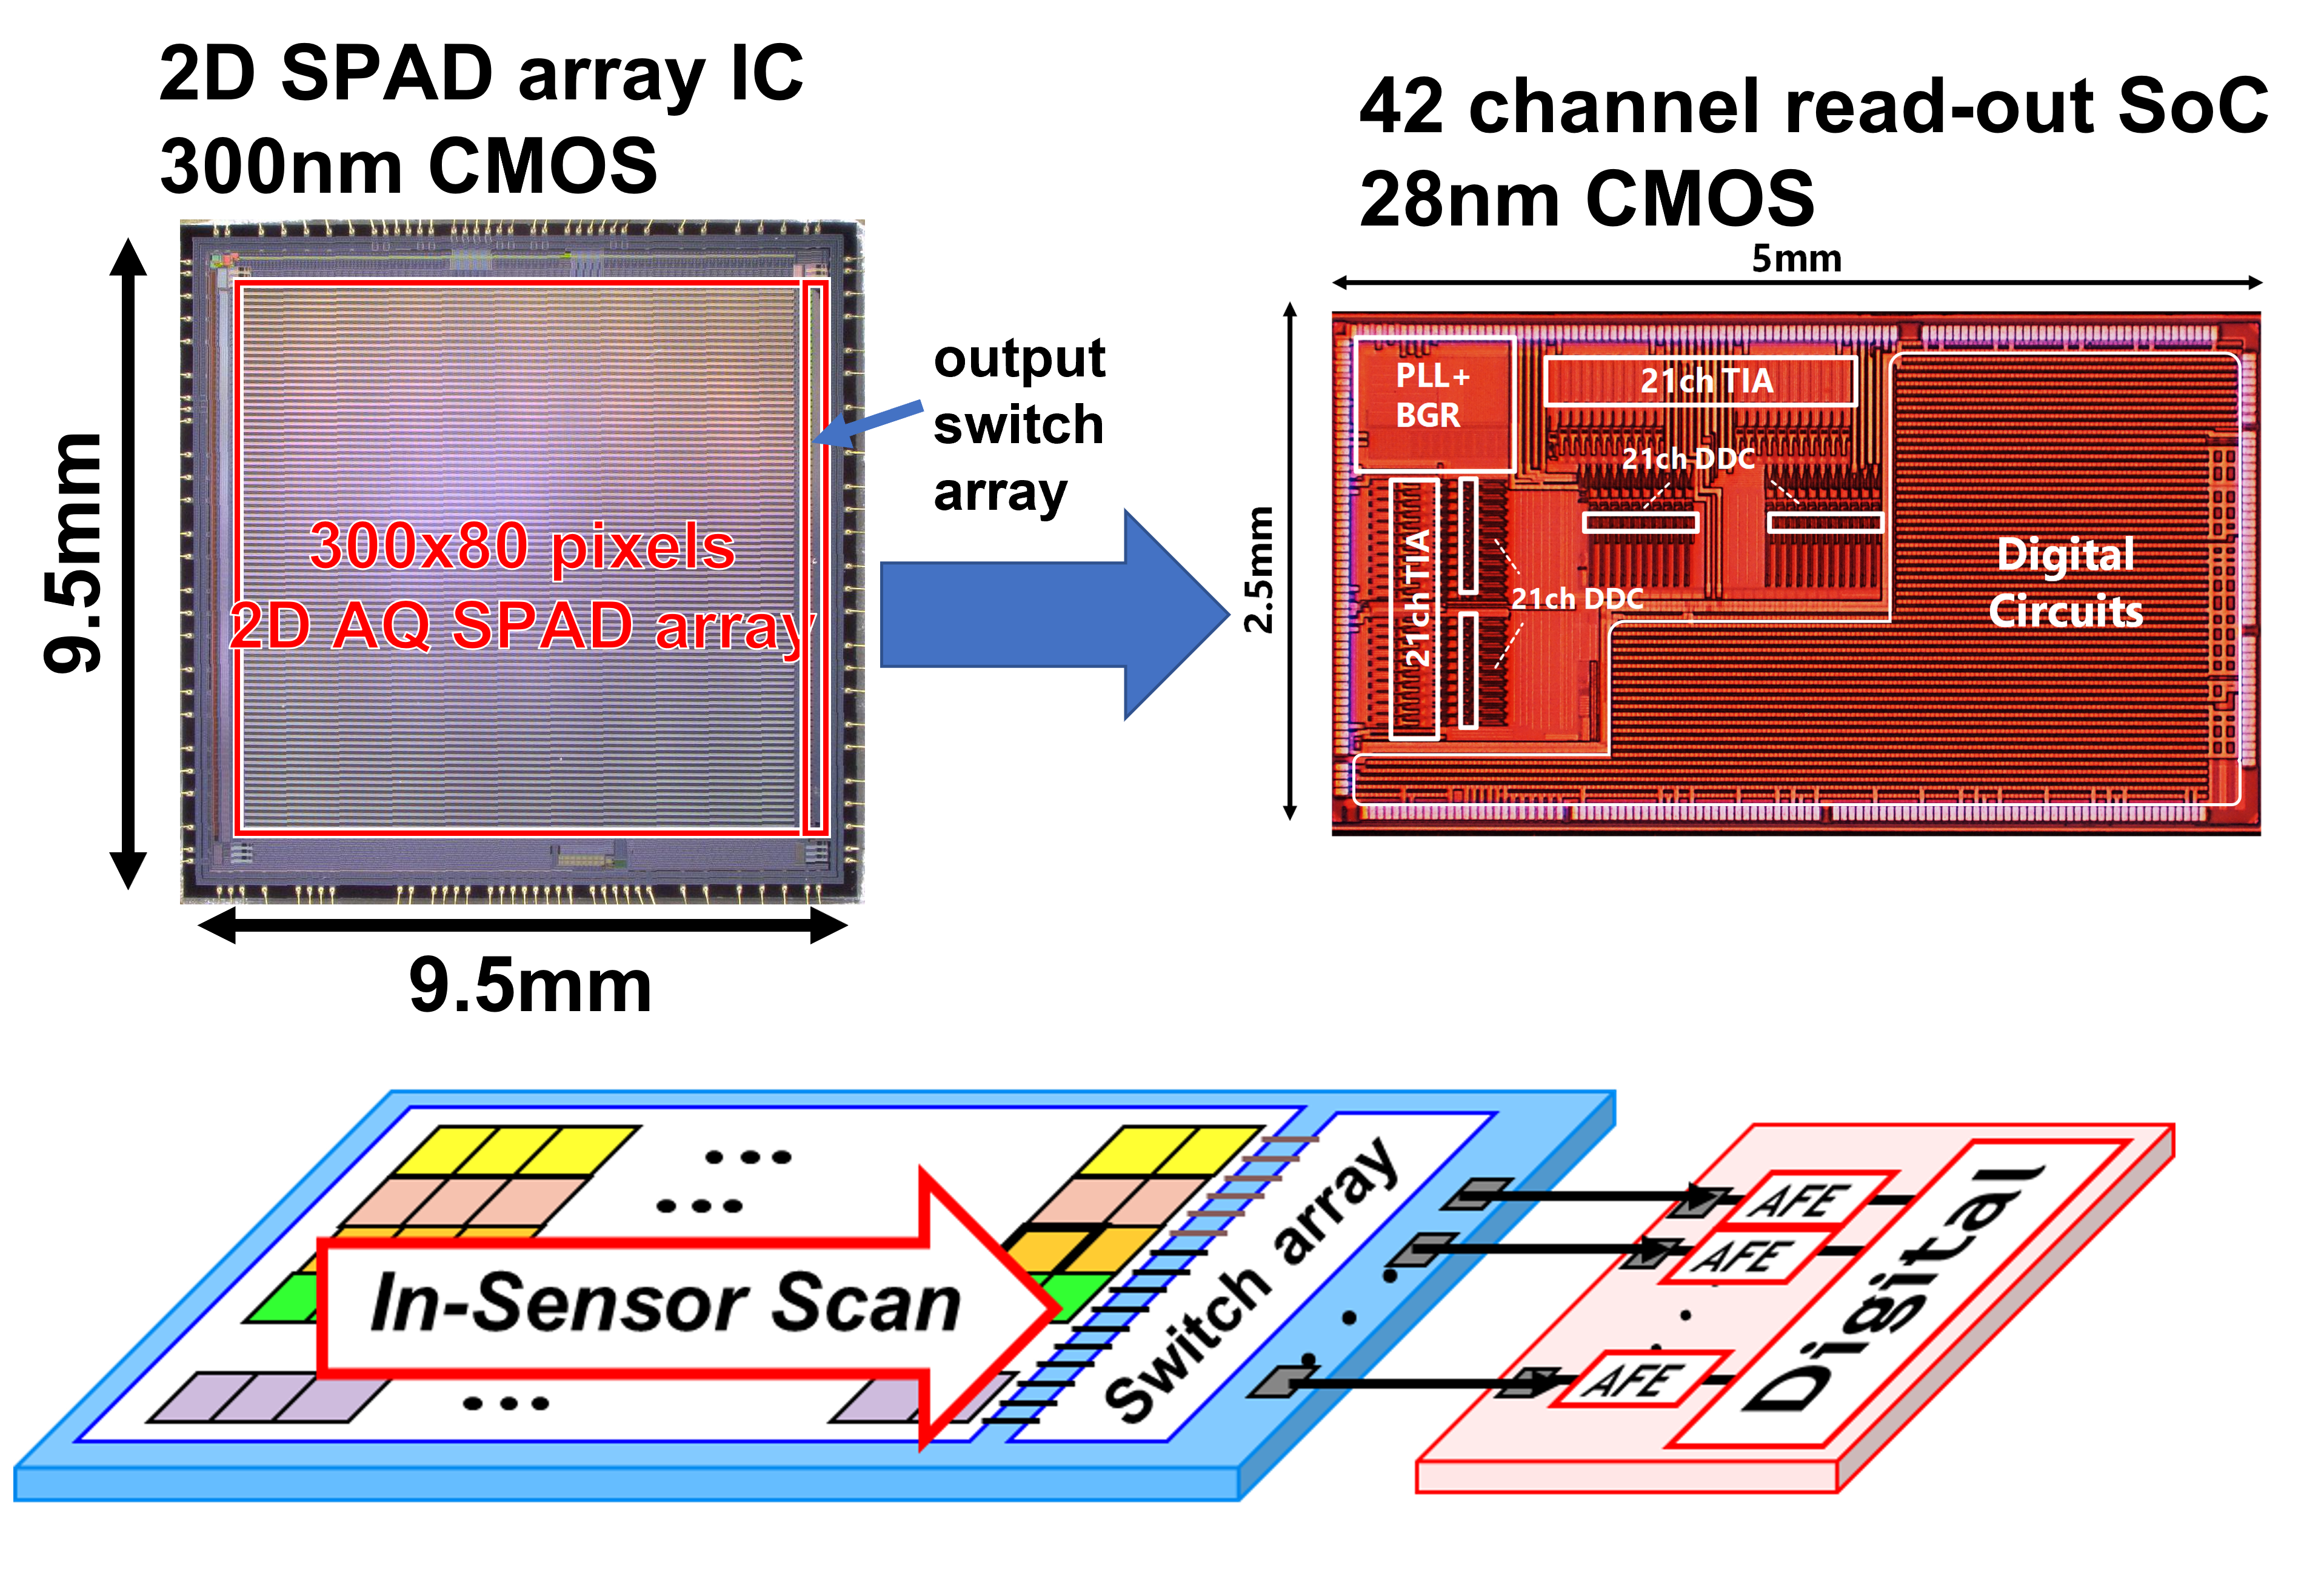
\includegraphics[width=0.5\textwidth]{figs/tan.png}
  \caption{2 chip system \cite{ta20202d}}
\label{tan}
\end{figure}

\begin{figure}[!t]
\centering
 \includegraphics[width=0.4\textwidth]{figs/toshiba-proto.png}
  \caption{2 chip system \cite{ieee}}
\label{ieee}
\end{figure}

NiclassとToshibaでは両方ともラスタースキャンを行うためにFig.\ref{raster}のようなセットアップをとっており、使用していたSPADアレーは1Dアレーであった。
このようなアプローチではSPAD数を抑えられるものの、受光光と送信レーザビーム両方の走査が必要であり可動部が非常に多くなってしまう。
そこでFig.\ref{tan}\cite{ta20202d}では受光を2D SPADアレーで行い、ラスタースキャンを受光アレー内の制御で行うIn sensor scanningによって受光側の可動部をなくす。
LiDARでは特に受光側のビーム走査は開口率が大きいため複雑な光学系と走査機構が必要になるが、In Sensor Scanningによってそれらを大幅に単純化できるためLiDAR筐体を著しく小さくする(Fig.\ref{ieee})。
加えてSPADをトランジスタにてリセットするアクディブクエンチング技術を使用することでクエンチング時間を短くし、画素あたりに必要なSPAD数を低減している。


\subsection{3Dインテグレーションアプローチ}
\begin{figure}[!t]
\centering
 \includegraphics[width=0.5\textwidth]{figs/sonypix.png}
  \caption{3D integrated SPADs \cite{ito2020back}}
\label{sony3d}
\end{figure}

\begin{figure}[!t]
\centering
 \includegraphics[width=0.5\textwidth]{figs/sony}
  \caption{3D integrated LiDAR SoC \cite{kumagai2021189x600}}
\label{sony}
\end{figure}

上記の研究のようにSPADと信号処理チップを分離し各々適したプロセスで製造することで性能向上を図れる。一方で画素数が増えてくるとチップ間接続が課題となってしまいスケーラビリティを失ってしまう。またSiPM接続によってTDCに対し面積効率の悪いADCは必要となってしまう。そこでSonyはイメージセンサで利用されている3Dインテグレーションアプローチを用いたLiDAR SoCを発表している(Fig.\ref{sony3d}, \ref{sony})。3DインテグレーションによってSPADと信号処理それぞれを好適なプロセス(それぞれ90nmと40nm)で製造できる。そのうえ高密度なチップ間IOを大量に使用することで100,000もの大量のSPADの配線も容易に結線できる。 
加えてもう一つのブレイクスルーはSPADにマイクロレンズとBSI技術を適応している点である。これもイメージセンサのPD高感度化では一般的な技術であるが、SPADに適応することでPDEが905nm波長にて22\%と大幅な向上を達成し高性能化に寄与している。

\subsection{Future directions}
\begin{table*}[!t]
\centering
\caption{First-gen vs Next-gen lidars}
 \includegraphics[width=0.9\textwidth]{figs/performance.png}
\label{perf}
\end{table*}
最後に上記で触れたLiDARの性能比較をTable\ref{perf}にて実施する。いずれもスキャン方式や解像度が異なるため直接的な比較を行うのは難しい。例えばMEMSミラーは回転ミラーに対しSNRは低くなってしまうため、LiDAR距離としては不利になる。そのため性能の絶対値よりも導入しているテクノロジーの進歩性によって評価するのが良いと考えている。

今後のLiDARの発展には商用と研究で大きく2つの方向性がある。商用には3Dインテグレーションやより微細プロセスを用いることで更にSPAD性能やDSP性能を向上させることでdToF車載LiDARの性能発展が見込まれる。そして十分に信頼性や量産性が確保されたのであれば市販車のADASシステムに搭載される日も遠くないと筆者は考えている。

また研究としては1550nm LiDARに大きな可能性が残されている。特にdToF LiDARは悪意を持った攻撃者にハッキングされる危険性があり\cite{sun2020towards, cao2019adversarial}、これを防ぐことのできるFMCW LiDARに期待が集まっている\cite{aptivpatent}。またシリコンフォトニクスを用いたLiDARは送信側のレーザ走査をもsolid-state化することが期待され研究の発展動向に注目している\cite{poulton2017coherent,chung202119}。

\section{Conclusions}
% 書く
自動運転システムの距離センサとして中核的な役割を果たすdTOF 車載用LiDARについて解説とreviewを行った。
黎明期の第一世代LiDAR、そしてシステムをチップ上に集積することでコストと性能を大きく改善した次世代LiDARについてreviewを行った。
特に次世代LiDARの主な進歩要因を受光素子、読み出し回路、及び信号処理部の集積化と捉えそれぞれの回路システムについてディスカッションを行った。加えて2チップアプローチ、2D SPADアレー、そして3DインテグレーションLiDARといった最新の研究例のディスカッションを行うことで本分野の最新の発展について議論した。

\section*{Acknowledgements}
This work was supported in part by the JST CREST program under Grant JPMJCR21D2, and in part by the Japan Society for the Promotion of Science (JSPS) KAKENHI, under Grant 21K20413.

\bibliographystyle{IEEEbib}
\bibliography{main}


\begin{IEEEbiography}
[{\includegraphics[width=1in,height=1.25in,clip,keepaspectratio]{bio/1.jpg}}]{Kentaro Yoshioka}
received his BS, MS, Ph.D degrees from Keio University, Japan. Currently, he is an Assistant Professor at Keio University. He worked with Toshiba during 2014-2021, developing circuitry for WiFi and LiDAR SoCs. During 2017-2018, he had been a visiting scholar at Stanford University, exploring efficient machine learning hardware and algorithms. 

Currently, Dr. Yoshioka serves as a technical program member of Symp. VLSI circuits conference. He was the recipient of ASP-DAC 2013 Special Feature Award, the A-SSCC 2012 Best Design Award, and 1st place winner of Kaggle 2020 Prostate Cancer Grade Assessment (PANDA) Challenge.
\end{IEEEbiography}

\end{document}
